\documentclass{article}%
\usepackage[T1]{fontenc}%
\usepackage[utf8]{inputenc}%
\usepackage{lmodern}%
\usepackage{textcomp}%
\usepackage{lastpage}%
\usepackage{xcolor}%
\usepackage{float}%
\usepackage[top=2.5cm, left=2.5cm, right=2.5cm]{geometry}%
\usepackage{tikz}%
%
\definecolor{pushcolor}{HTML}{a5f56c}%
%
\begin{document}%
\normalsize%
\section{Stack Implementation Using Two Queues}%
\label{sec:StackImplementationUsingTwoQueues}%
A stack is a LIFO (Last In, First Out) data structure, while a queue is a FIFO (First In, First Out) data structure. The challenge here is to simulate stack behavior using queues. We can use two queues, q1 and q2, to implement a stack. The key idea is to:

Push operation:
1. Enqueue the new element into q2.
2. Dequeue all elements from q1 and enqueue them into q2.
3. Swap the names of q1 and q2.

Pop operation:
1. Dequeue and return the front element of q1.

%
\section{After pushing 52}%
\label{sec:Afterpushing52}%


\begin{figure}[H]%
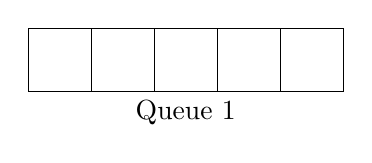
\begin{tikzpicture}%
\node[draw, rectangle, minimum width=0.8cm, minimum height=0.8cm, fill=white, font=\fontsize{0.24cm}{0.288cm}\selectfont] at (0.0, 0) {};%
\node[draw, rectangle, minimum width=0.8cm, minimum height=0.8cm, fill=white, font=\fontsize{0.24cm}{0.288cm}\selectfont] at (0.8, 0) {};%
\node[draw, rectangle, minimum width=0.8cm, minimum height=0.8cm, fill=white, font=\fontsize{0.24cm}{0.288cm}\selectfont] at (1.6, 0) {};%
\node[draw, rectangle, minimum width=0.8cm, minimum height=0.8cm, fill=white, font=\fontsize{0.24cm}{0.288cm}\selectfont] at (2.4000000000000004, 0) {};%
\node[draw, rectangle, minimum width=0.8cm, minimum height=0.8cm, fill=white, font=\fontsize{0.24cm}{0.288cm}\selectfont] at (3.2, 0) {};%
\node[below] at (1.6, -0.4) {Queue 1};%
\end{tikzpicture}%
\end{figure}

%


\begin{figure}[H]%
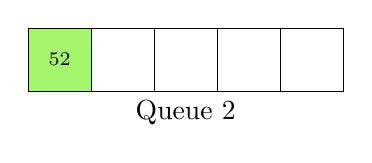
\begin{tikzpicture}%
\node[draw, rectangle, minimum width=0.8cm, minimum height=0.8cm, fill=pushcolor, font=\fontsize{0.24cm}{0.288cm}\selectfont] at (0.0, 0) {52};%
\node[draw, rectangle, minimum width=0.8cm, minimum height=0.8cm, fill=white, font=\fontsize{0.24cm}{0.288cm}\selectfont] at (0.8, 0) {};%
\node[draw, rectangle, minimum width=0.8cm, minimum height=0.8cm, fill=white, font=\fontsize{0.24cm}{0.288cm}\selectfont] at (1.6, 0) {};%
\node[draw, rectangle, minimum width=0.8cm, minimum height=0.8cm, fill=white, font=\fontsize{0.24cm}{0.288cm}\selectfont] at (2.4000000000000004, 0) {};%
\node[draw, rectangle, minimum width=0.8cm, minimum height=0.8cm, fill=white, font=\fontsize{0.24cm}{0.288cm}\selectfont] at (3.2, 0) {};%
\node[below] at (1.6, -0.4) {Queue 2};%
\end{tikzpicture}%
\end{figure}

%
\section{Final state after pushing 52}%
\label{sec:Finalstateafterpushing52}%


\begin{figure}[H]%
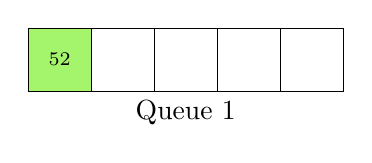
\begin{tikzpicture}%
\node[draw, rectangle, minimum width=0.8cm, minimum height=0.8cm, fill=pushcolor, font=\fontsize{0.24cm}{0.288cm}\selectfont] at (0.0, 0) {52};%
\node[draw, rectangle, minimum width=0.8cm, minimum height=0.8cm, fill=white, font=\fontsize{0.24cm}{0.288cm}\selectfont] at (0.8, 0) {};%
\node[draw, rectangle, minimum width=0.8cm, minimum height=0.8cm, fill=white, font=\fontsize{0.24cm}{0.288cm}\selectfont] at (1.6, 0) {};%
\node[draw, rectangle, minimum width=0.8cm, minimum height=0.8cm, fill=white, font=\fontsize{0.24cm}{0.288cm}\selectfont] at (2.4000000000000004, 0) {};%
\node[draw, rectangle, minimum width=0.8cm, minimum height=0.8cm, fill=white, font=\fontsize{0.24cm}{0.288cm}\selectfont] at (3.2, 0) {};%
\node[below] at (1.6, -0.4) {Queue 1};%
\end{tikzpicture}%
\end{figure}

%


\begin{figure}[H]%
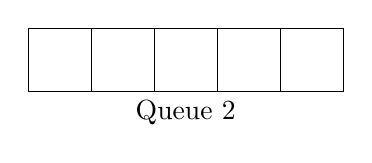
\begin{tikzpicture}%
\node[draw, rectangle, minimum width=0.8cm, minimum height=0.8cm, fill=white, font=\fontsize{0.24cm}{0.288cm}\selectfont] at (0.0, 0) {};%
\node[draw, rectangle, minimum width=0.8cm, minimum height=0.8cm, fill=white, font=\fontsize{0.24cm}{0.288cm}\selectfont] at (0.8, 0) {};%
\node[draw, rectangle, minimum width=0.8cm, minimum height=0.8cm, fill=white, font=\fontsize{0.24cm}{0.288cm}\selectfont] at (1.6, 0) {};%
\node[draw, rectangle, minimum width=0.8cm, minimum height=0.8cm, fill=white, font=\fontsize{0.24cm}{0.288cm}\selectfont] at (2.4000000000000004, 0) {};%
\node[draw, rectangle, minimum width=0.8cm, minimum height=0.8cm, fill=white, font=\fontsize{0.24cm}{0.288cm}\selectfont] at (3.2, 0) {};%
\node[below] at (1.6, -0.4) {Queue 2};%
\end{tikzpicture}%
\end{figure}

%
\section{After pushing 10}%
\label{sec:Afterpushing10}%


\begin{figure}[H]%
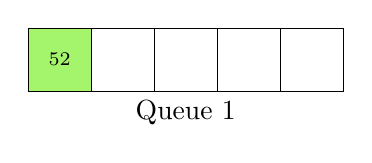
\begin{tikzpicture}%
\node[draw, rectangle, minimum width=0.8cm, minimum height=0.8cm, fill=pushcolor, font=\fontsize{0.24cm}{0.288cm}\selectfont] at (0.0, 0) {52};%
\node[draw, rectangle, minimum width=0.8cm, minimum height=0.8cm, fill=white, font=\fontsize{0.24cm}{0.288cm}\selectfont] at (0.8, 0) {};%
\node[draw, rectangle, minimum width=0.8cm, minimum height=0.8cm, fill=white, font=\fontsize{0.24cm}{0.288cm}\selectfont] at (1.6, 0) {};%
\node[draw, rectangle, minimum width=0.8cm, minimum height=0.8cm, fill=white, font=\fontsize{0.24cm}{0.288cm}\selectfont] at (2.4000000000000004, 0) {};%
\node[draw, rectangle, minimum width=0.8cm, minimum height=0.8cm, fill=white, font=\fontsize{0.24cm}{0.288cm}\selectfont] at (3.2, 0) {};%
\node[below] at (1.6, -0.4) {Queue 1};%
\end{tikzpicture}%
\end{figure}

%


\begin{figure}[H]%
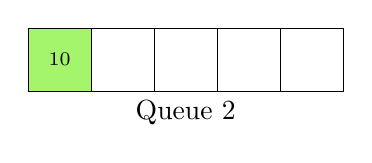
\begin{tikzpicture}%
\node[draw, rectangle, minimum width=0.8cm, minimum height=0.8cm, fill=pushcolor, font=\fontsize{0.24cm}{0.288cm}\selectfont] at (0.0, 0) {10};%
\node[draw, rectangle, minimum width=0.8cm, minimum height=0.8cm, fill=white, font=\fontsize{0.24cm}{0.288cm}\selectfont] at (0.8, 0) {};%
\node[draw, rectangle, minimum width=0.8cm, minimum height=0.8cm, fill=white, font=\fontsize{0.24cm}{0.288cm}\selectfont] at (1.6, 0) {};%
\node[draw, rectangle, minimum width=0.8cm, minimum height=0.8cm, fill=white, font=\fontsize{0.24cm}{0.288cm}\selectfont] at (2.4000000000000004, 0) {};%
\node[draw, rectangle, minimum width=0.8cm, minimum height=0.8cm, fill=white, font=\fontsize{0.24cm}{0.288cm}\selectfont] at (3.2, 0) {};%
\node[below] at (1.6, -0.4) {Queue 2};%
\end{tikzpicture}%
\end{figure}

%
\section{During push (transferring elements)}%
\label{sec:Duringpush(transferringelements)}%


\begin{figure}[H]%
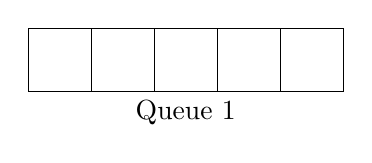
\begin{tikzpicture}%
\node[draw, rectangle, minimum width=0.8cm, minimum height=0.8cm, fill=white, font=\fontsize{0.24cm}{0.288cm}\selectfont] at (0.0, 0) {};%
\node[draw, rectangle, minimum width=0.8cm, minimum height=0.8cm, fill=white, font=\fontsize{0.24cm}{0.288cm}\selectfont] at (0.8, 0) {};%
\node[draw, rectangle, minimum width=0.8cm, minimum height=0.8cm, fill=white, font=\fontsize{0.24cm}{0.288cm}\selectfont] at (1.6, 0) {};%
\node[draw, rectangle, minimum width=0.8cm, minimum height=0.8cm, fill=white, font=\fontsize{0.24cm}{0.288cm}\selectfont] at (2.4000000000000004, 0) {};%
\node[draw, rectangle, minimum width=0.8cm, minimum height=0.8cm, fill=white, font=\fontsize{0.24cm}{0.288cm}\selectfont] at (3.2, 0) {};%
\node[below] at (1.6, -0.4) {Queue 1};%
\end{tikzpicture}%
\end{figure}

%


\begin{figure}[H]%
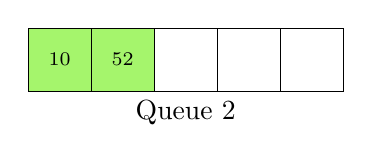
\begin{tikzpicture}%
\node[draw, rectangle, minimum width=0.8cm, minimum height=0.8cm, fill=pushcolor, font=\fontsize{0.24cm}{0.288cm}\selectfont] at (0.0, 0) {10};%
\node[draw, rectangle, minimum width=0.8cm, minimum height=0.8cm, fill=pushcolor, font=\fontsize{0.24cm}{0.288cm}\selectfont] at (0.8, 0) {52};%
\node[draw, rectangle, minimum width=0.8cm, minimum height=0.8cm, fill=white, font=\fontsize{0.24cm}{0.288cm}\selectfont] at (1.6, 0) {};%
\node[draw, rectangle, minimum width=0.8cm, minimum height=0.8cm, fill=white, font=\fontsize{0.24cm}{0.288cm}\selectfont] at (2.4000000000000004, 0) {};%
\node[draw, rectangle, minimum width=0.8cm, minimum height=0.8cm, fill=white, font=\fontsize{0.24cm}{0.288cm}\selectfont] at (3.2, 0) {};%
\node[below] at (1.6, -0.4) {Queue 2};%
\end{tikzpicture}%
\end{figure}

%
\section{Final state after pushing 10}%
\label{sec:Finalstateafterpushing10}%


\begin{figure}[H]%
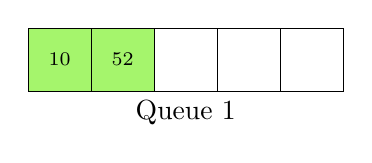
\begin{tikzpicture}%
\node[draw, rectangle, minimum width=0.8cm, minimum height=0.8cm, fill=pushcolor, font=\fontsize{0.24cm}{0.288cm}\selectfont] at (0.0, 0) {10};%
\node[draw, rectangle, minimum width=0.8cm, minimum height=0.8cm, fill=pushcolor, font=\fontsize{0.24cm}{0.288cm}\selectfont] at (0.8, 0) {52};%
\node[draw, rectangle, minimum width=0.8cm, minimum height=0.8cm, fill=white, font=\fontsize{0.24cm}{0.288cm}\selectfont] at (1.6, 0) {};%
\node[draw, rectangle, minimum width=0.8cm, minimum height=0.8cm, fill=white, font=\fontsize{0.24cm}{0.288cm}\selectfont] at (2.4000000000000004, 0) {};%
\node[draw, rectangle, minimum width=0.8cm, minimum height=0.8cm, fill=white, font=\fontsize{0.24cm}{0.288cm}\selectfont] at (3.2, 0) {};%
\node[below] at (1.6, -0.4) {Queue 1};%
\end{tikzpicture}%
\end{figure}

%


\begin{figure}[H]%
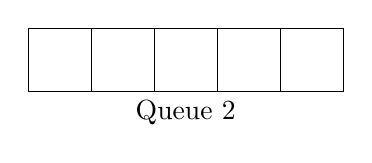
\begin{tikzpicture}%
\node[draw, rectangle, minimum width=0.8cm, minimum height=0.8cm, fill=white, font=\fontsize{0.24cm}{0.288cm}\selectfont] at (0.0, 0) {};%
\node[draw, rectangle, minimum width=0.8cm, minimum height=0.8cm, fill=white, font=\fontsize{0.24cm}{0.288cm}\selectfont] at (0.8, 0) {};%
\node[draw, rectangle, minimum width=0.8cm, minimum height=0.8cm, fill=white, font=\fontsize{0.24cm}{0.288cm}\selectfont] at (1.6, 0) {};%
\node[draw, rectangle, minimum width=0.8cm, minimum height=0.8cm, fill=white, font=\fontsize{0.24cm}{0.288cm}\selectfont] at (2.4000000000000004, 0) {};%
\node[draw, rectangle, minimum width=0.8cm, minimum height=0.8cm, fill=white, font=\fontsize{0.24cm}{0.288cm}\selectfont] at (3.2, 0) {};%
\node[below] at (1.6, -0.4) {Queue 2};%
\end{tikzpicture}%
\end{figure}

%
\section{Final state after popping 10}%
\label{sec:Finalstateafterpopping10}%


\begin{figure}[H]%
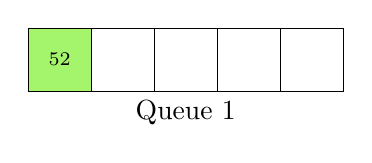
\begin{tikzpicture}%
\node[draw, rectangle, minimum width=0.8cm, minimum height=0.8cm, fill=pushcolor, font=\fontsize{0.24cm}{0.288cm}\selectfont] at (0.0, 0) {52};%
\node[draw, rectangle, minimum width=0.8cm, minimum height=0.8cm, fill=white, font=\fontsize{0.24cm}{0.288cm}\selectfont] at (0.8, 0) {};%
\node[draw, rectangle, minimum width=0.8cm, minimum height=0.8cm, fill=white, font=\fontsize{0.24cm}{0.288cm}\selectfont] at (1.6, 0) {};%
\node[draw, rectangle, minimum width=0.8cm, minimum height=0.8cm, fill=white, font=\fontsize{0.24cm}{0.288cm}\selectfont] at (2.4000000000000004, 0) {};%
\node[draw, rectangle, minimum width=0.8cm, minimum height=0.8cm, fill=white, font=\fontsize{0.24cm}{0.288cm}\selectfont] at (3.2, 0) {};%
\node[below] at (1.6, -0.4) {Queue 1};%
\end{tikzpicture}%
\end{figure}

%


\begin{figure}[H]%
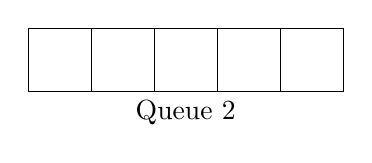
\begin{tikzpicture}%
\node[draw, rectangle, minimum width=0.8cm, minimum height=0.8cm, fill=white, font=\fontsize{0.24cm}{0.288cm}\selectfont] at (0.0, 0) {};%
\node[draw, rectangle, minimum width=0.8cm, minimum height=0.8cm, fill=white, font=\fontsize{0.24cm}{0.288cm}\selectfont] at (0.8, 0) {};%
\node[draw, rectangle, minimum width=0.8cm, minimum height=0.8cm, fill=white, font=\fontsize{0.24cm}{0.288cm}\selectfont] at (1.6, 0) {};%
\node[draw, rectangle, minimum width=0.8cm, minimum height=0.8cm, fill=white, font=\fontsize{0.24cm}{0.288cm}\selectfont] at (2.4000000000000004, 0) {};%
\node[draw, rectangle, minimum width=0.8cm, minimum height=0.8cm, fill=white, font=\fontsize{0.24cm}{0.288cm}\selectfont] at (3.2, 0) {};%
\node[below] at (1.6, -0.4) {Queue 2};%
\end{tikzpicture}%
\end{figure}

%
\section{After pushing 15}%
\label{sec:Afterpushing15}%


\begin{figure}[H]%
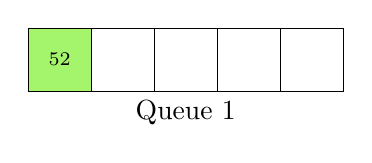
\begin{tikzpicture}%
\node[draw, rectangle, minimum width=0.8cm, minimum height=0.8cm, fill=pushcolor, font=\fontsize{0.24cm}{0.288cm}\selectfont] at (0.0, 0) {52};%
\node[draw, rectangle, minimum width=0.8cm, minimum height=0.8cm, fill=white, font=\fontsize{0.24cm}{0.288cm}\selectfont] at (0.8, 0) {};%
\node[draw, rectangle, minimum width=0.8cm, minimum height=0.8cm, fill=white, font=\fontsize{0.24cm}{0.288cm}\selectfont] at (1.6, 0) {};%
\node[draw, rectangle, minimum width=0.8cm, minimum height=0.8cm, fill=white, font=\fontsize{0.24cm}{0.288cm}\selectfont] at (2.4000000000000004, 0) {};%
\node[draw, rectangle, minimum width=0.8cm, minimum height=0.8cm, fill=white, font=\fontsize{0.24cm}{0.288cm}\selectfont] at (3.2, 0) {};%
\node[below] at (1.6, -0.4) {Queue 1};%
\end{tikzpicture}%
\end{figure}

%


\begin{figure}[H]%
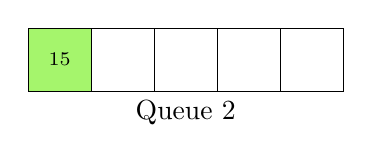
\begin{tikzpicture}%
\node[draw, rectangle, minimum width=0.8cm, minimum height=0.8cm, fill=pushcolor, font=\fontsize{0.24cm}{0.288cm}\selectfont] at (0.0, 0) {15};%
\node[draw, rectangle, minimum width=0.8cm, minimum height=0.8cm, fill=white, font=\fontsize{0.24cm}{0.288cm}\selectfont] at (0.8, 0) {};%
\node[draw, rectangle, minimum width=0.8cm, minimum height=0.8cm, fill=white, font=\fontsize{0.24cm}{0.288cm}\selectfont] at (1.6, 0) {};%
\node[draw, rectangle, minimum width=0.8cm, minimum height=0.8cm, fill=white, font=\fontsize{0.24cm}{0.288cm}\selectfont] at (2.4000000000000004, 0) {};%
\node[draw, rectangle, minimum width=0.8cm, minimum height=0.8cm, fill=white, font=\fontsize{0.24cm}{0.288cm}\selectfont] at (3.2, 0) {};%
\node[below] at (1.6, -0.4) {Queue 2};%
\end{tikzpicture}%
\end{figure}

%
\section{During push (transferring elements)}%
\label{sec:Duringpush(transferringelements)}%


\begin{figure}[H]%
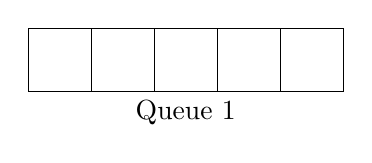
\begin{tikzpicture}%
\node[draw, rectangle, minimum width=0.8cm, minimum height=0.8cm, fill=white, font=\fontsize{0.24cm}{0.288cm}\selectfont] at (0.0, 0) {};%
\node[draw, rectangle, minimum width=0.8cm, minimum height=0.8cm, fill=white, font=\fontsize{0.24cm}{0.288cm}\selectfont] at (0.8, 0) {};%
\node[draw, rectangle, minimum width=0.8cm, minimum height=0.8cm, fill=white, font=\fontsize{0.24cm}{0.288cm}\selectfont] at (1.6, 0) {};%
\node[draw, rectangle, minimum width=0.8cm, minimum height=0.8cm, fill=white, font=\fontsize{0.24cm}{0.288cm}\selectfont] at (2.4000000000000004, 0) {};%
\node[draw, rectangle, minimum width=0.8cm, minimum height=0.8cm, fill=white, font=\fontsize{0.24cm}{0.288cm}\selectfont] at (3.2, 0) {};%
\node[below] at (1.6, -0.4) {Queue 1};%
\end{tikzpicture}%
\end{figure}

%


\begin{figure}[H]%
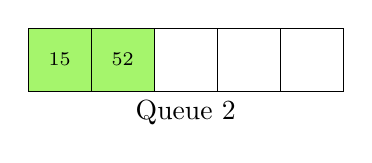
\begin{tikzpicture}%
\node[draw, rectangle, minimum width=0.8cm, minimum height=0.8cm, fill=pushcolor, font=\fontsize{0.24cm}{0.288cm}\selectfont] at (0.0, 0) {15};%
\node[draw, rectangle, minimum width=0.8cm, minimum height=0.8cm, fill=pushcolor, font=\fontsize{0.24cm}{0.288cm}\selectfont] at (0.8, 0) {52};%
\node[draw, rectangle, minimum width=0.8cm, minimum height=0.8cm, fill=white, font=\fontsize{0.24cm}{0.288cm}\selectfont] at (1.6, 0) {};%
\node[draw, rectangle, minimum width=0.8cm, minimum height=0.8cm, fill=white, font=\fontsize{0.24cm}{0.288cm}\selectfont] at (2.4000000000000004, 0) {};%
\node[draw, rectangle, minimum width=0.8cm, minimum height=0.8cm, fill=white, font=\fontsize{0.24cm}{0.288cm}\selectfont] at (3.2, 0) {};%
\node[below] at (1.6, -0.4) {Queue 2};%
\end{tikzpicture}%
\end{figure}

%
\section{Final state after pushing 15}%
\label{sec:Finalstateafterpushing15}%


\begin{figure}[H]%
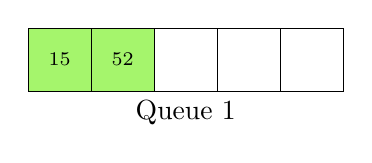
\begin{tikzpicture}%
\node[draw, rectangle, minimum width=0.8cm, minimum height=0.8cm, fill=pushcolor, font=\fontsize{0.24cm}{0.288cm}\selectfont] at (0.0, 0) {15};%
\node[draw, rectangle, minimum width=0.8cm, minimum height=0.8cm, fill=pushcolor, font=\fontsize{0.24cm}{0.288cm}\selectfont] at (0.8, 0) {52};%
\node[draw, rectangle, minimum width=0.8cm, minimum height=0.8cm, fill=white, font=\fontsize{0.24cm}{0.288cm}\selectfont] at (1.6, 0) {};%
\node[draw, rectangle, minimum width=0.8cm, minimum height=0.8cm, fill=white, font=\fontsize{0.24cm}{0.288cm}\selectfont] at (2.4000000000000004, 0) {};%
\node[draw, rectangle, minimum width=0.8cm, minimum height=0.8cm, fill=white, font=\fontsize{0.24cm}{0.288cm}\selectfont] at (3.2, 0) {};%
\node[below] at (1.6, -0.4) {Queue 1};%
\end{tikzpicture}%
\end{figure}

%


\begin{figure}[H]%
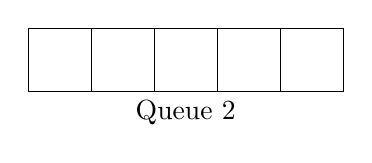
\begin{tikzpicture}%
\node[draw, rectangle, minimum width=0.8cm, minimum height=0.8cm, fill=white, font=\fontsize{0.24cm}{0.288cm}\selectfont] at (0.0, 0) {};%
\node[draw, rectangle, minimum width=0.8cm, minimum height=0.8cm, fill=white, font=\fontsize{0.24cm}{0.288cm}\selectfont] at (0.8, 0) {};%
\node[draw, rectangle, minimum width=0.8cm, minimum height=0.8cm, fill=white, font=\fontsize{0.24cm}{0.288cm}\selectfont] at (1.6, 0) {};%
\node[draw, rectangle, minimum width=0.8cm, minimum height=0.8cm, fill=white, font=\fontsize{0.24cm}{0.288cm}\selectfont] at (2.4000000000000004, 0) {};%
\node[draw, rectangle, minimum width=0.8cm, minimum height=0.8cm, fill=white, font=\fontsize{0.24cm}{0.288cm}\selectfont] at (3.2, 0) {};%
\node[below] at (1.6, -0.4) {Queue 2};%
\end{tikzpicture}%
\end{figure}

%
\section{After pushing 20}%
\label{sec:Afterpushing20}%


\begin{figure}[H]%
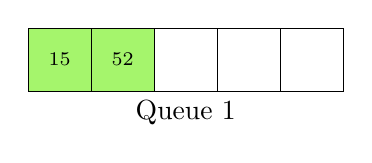
\begin{tikzpicture}%
\node[draw, rectangle, minimum width=0.8cm, minimum height=0.8cm, fill=pushcolor, font=\fontsize{0.24cm}{0.288cm}\selectfont] at (0.0, 0) {15};%
\node[draw, rectangle, minimum width=0.8cm, minimum height=0.8cm, fill=pushcolor, font=\fontsize{0.24cm}{0.288cm}\selectfont] at (0.8, 0) {52};%
\node[draw, rectangle, minimum width=0.8cm, minimum height=0.8cm, fill=white, font=\fontsize{0.24cm}{0.288cm}\selectfont] at (1.6, 0) {};%
\node[draw, rectangle, minimum width=0.8cm, minimum height=0.8cm, fill=white, font=\fontsize{0.24cm}{0.288cm}\selectfont] at (2.4000000000000004, 0) {};%
\node[draw, rectangle, minimum width=0.8cm, minimum height=0.8cm, fill=white, font=\fontsize{0.24cm}{0.288cm}\selectfont] at (3.2, 0) {};%
\node[below] at (1.6, -0.4) {Queue 1};%
\end{tikzpicture}%
\end{figure}

%


\begin{figure}[H]%
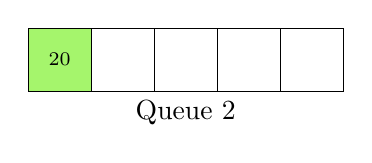
\begin{tikzpicture}%
\node[draw, rectangle, minimum width=0.8cm, minimum height=0.8cm, fill=pushcolor, font=\fontsize{0.24cm}{0.288cm}\selectfont] at (0.0, 0) {20};%
\node[draw, rectangle, minimum width=0.8cm, minimum height=0.8cm, fill=white, font=\fontsize{0.24cm}{0.288cm}\selectfont] at (0.8, 0) {};%
\node[draw, rectangle, minimum width=0.8cm, minimum height=0.8cm, fill=white, font=\fontsize{0.24cm}{0.288cm}\selectfont] at (1.6, 0) {};%
\node[draw, rectangle, minimum width=0.8cm, minimum height=0.8cm, fill=white, font=\fontsize{0.24cm}{0.288cm}\selectfont] at (2.4000000000000004, 0) {};%
\node[draw, rectangle, minimum width=0.8cm, minimum height=0.8cm, fill=white, font=\fontsize{0.24cm}{0.288cm}\selectfont] at (3.2, 0) {};%
\node[below] at (1.6, -0.4) {Queue 2};%
\end{tikzpicture}%
\end{figure}

%
\section{During push (transferring elements)}%
\label{sec:Duringpush(transferringelements)}%


\begin{figure}[H]%
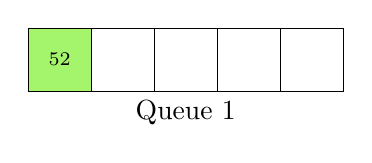
\begin{tikzpicture}%
\node[draw, rectangle, minimum width=0.8cm, minimum height=0.8cm, fill=pushcolor, font=\fontsize{0.24cm}{0.288cm}\selectfont] at (0.0, 0) {52};%
\node[draw, rectangle, minimum width=0.8cm, minimum height=0.8cm, fill=white, font=\fontsize{0.24cm}{0.288cm}\selectfont] at (0.8, 0) {};%
\node[draw, rectangle, minimum width=0.8cm, minimum height=0.8cm, fill=white, font=\fontsize{0.24cm}{0.288cm}\selectfont] at (1.6, 0) {};%
\node[draw, rectangle, minimum width=0.8cm, minimum height=0.8cm, fill=white, font=\fontsize{0.24cm}{0.288cm}\selectfont] at (2.4000000000000004, 0) {};%
\node[draw, rectangle, minimum width=0.8cm, minimum height=0.8cm, fill=white, font=\fontsize{0.24cm}{0.288cm}\selectfont] at (3.2, 0) {};%
\node[below] at (1.6, -0.4) {Queue 1};%
\end{tikzpicture}%
\end{figure}

%


\begin{figure}[H]%
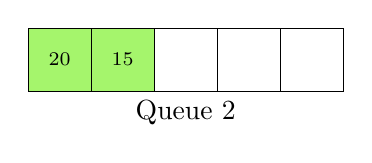
\begin{tikzpicture}%
\node[draw, rectangle, minimum width=0.8cm, minimum height=0.8cm, fill=pushcolor, font=\fontsize{0.24cm}{0.288cm}\selectfont] at (0.0, 0) {20};%
\node[draw, rectangle, minimum width=0.8cm, minimum height=0.8cm, fill=pushcolor, font=\fontsize{0.24cm}{0.288cm}\selectfont] at (0.8, 0) {15};%
\node[draw, rectangle, minimum width=0.8cm, minimum height=0.8cm, fill=white, font=\fontsize{0.24cm}{0.288cm}\selectfont] at (1.6, 0) {};%
\node[draw, rectangle, minimum width=0.8cm, minimum height=0.8cm, fill=white, font=\fontsize{0.24cm}{0.288cm}\selectfont] at (2.4000000000000004, 0) {};%
\node[draw, rectangle, minimum width=0.8cm, minimum height=0.8cm, fill=white, font=\fontsize{0.24cm}{0.288cm}\selectfont] at (3.2, 0) {};%
\node[below] at (1.6, -0.4) {Queue 2};%
\end{tikzpicture}%
\end{figure}

%
\section{During push (transferring elements)}%
\label{sec:Duringpush(transferringelements)}%


\begin{figure}[H]%
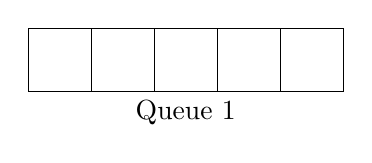
\begin{tikzpicture}%
\node[draw, rectangle, minimum width=0.8cm, minimum height=0.8cm, fill=white, font=\fontsize{0.24cm}{0.288cm}\selectfont] at (0.0, 0) {};%
\node[draw, rectangle, minimum width=0.8cm, minimum height=0.8cm, fill=white, font=\fontsize{0.24cm}{0.288cm}\selectfont] at (0.8, 0) {};%
\node[draw, rectangle, minimum width=0.8cm, minimum height=0.8cm, fill=white, font=\fontsize{0.24cm}{0.288cm}\selectfont] at (1.6, 0) {};%
\node[draw, rectangle, minimum width=0.8cm, minimum height=0.8cm, fill=white, font=\fontsize{0.24cm}{0.288cm}\selectfont] at (2.4000000000000004, 0) {};%
\node[draw, rectangle, minimum width=0.8cm, minimum height=0.8cm, fill=white, font=\fontsize{0.24cm}{0.288cm}\selectfont] at (3.2, 0) {};%
\node[below] at (1.6, -0.4) {Queue 1};%
\end{tikzpicture}%
\end{figure}

%


\begin{figure}[H]%
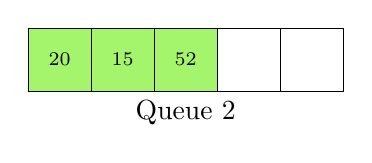
\begin{tikzpicture}%
\node[draw, rectangle, minimum width=0.8cm, minimum height=0.8cm, fill=pushcolor, font=\fontsize{0.24cm}{0.288cm}\selectfont] at (0.0, 0) {20};%
\node[draw, rectangle, minimum width=0.8cm, minimum height=0.8cm, fill=pushcolor, font=\fontsize{0.24cm}{0.288cm}\selectfont] at (0.8, 0) {15};%
\node[draw, rectangle, minimum width=0.8cm, minimum height=0.8cm, fill=pushcolor, font=\fontsize{0.24cm}{0.288cm}\selectfont] at (1.6, 0) {52};%
\node[draw, rectangle, minimum width=0.8cm, minimum height=0.8cm, fill=white, font=\fontsize{0.24cm}{0.288cm}\selectfont] at (2.4000000000000004, 0) {};%
\node[draw, rectangle, minimum width=0.8cm, minimum height=0.8cm, fill=white, font=\fontsize{0.24cm}{0.288cm}\selectfont] at (3.2, 0) {};%
\node[below] at (1.6, -0.4) {Queue 2};%
\end{tikzpicture}%
\end{figure}

%
\section{Final state after pushing 20}%
\label{sec:Finalstateafterpushing20}%


\begin{figure}[H]%
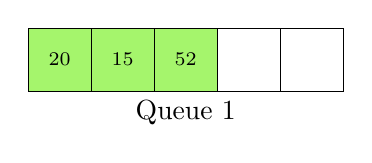
\begin{tikzpicture}%
\node[draw, rectangle, minimum width=0.8cm, minimum height=0.8cm, fill=pushcolor, font=\fontsize{0.24cm}{0.288cm}\selectfont] at (0.0, 0) {20};%
\node[draw, rectangle, minimum width=0.8cm, minimum height=0.8cm, fill=pushcolor, font=\fontsize{0.24cm}{0.288cm}\selectfont] at (0.8, 0) {15};%
\node[draw, rectangle, minimum width=0.8cm, minimum height=0.8cm, fill=pushcolor, font=\fontsize{0.24cm}{0.288cm}\selectfont] at (1.6, 0) {52};%
\node[draw, rectangle, minimum width=0.8cm, minimum height=0.8cm, fill=white, font=\fontsize{0.24cm}{0.288cm}\selectfont] at (2.4000000000000004, 0) {};%
\node[draw, rectangle, minimum width=0.8cm, minimum height=0.8cm, fill=white, font=\fontsize{0.24cm}{0.288cm}\selectfont] at (3.2, 0) {};%
\node[below] at (1.6, -0.4) {Queue 1};%
\end{tikzpicture}%
\end{figure}

%


\begin{figure}[H]%
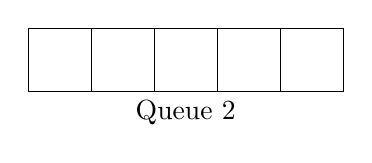
\begin{tikzpicture}%
\node[draw, rectangle, minimum width=0.8cm, minimum height=0.8cm, fill=white, font=\fontsize{0.24cm}{0.288cm}\selectfont] at (0.0, 0) {};%
\node[draw, rectangle, minimum width=0.8cm, minimum height=0.8cm, fill=white, font=\fontsize{0.24cm}{0.288cm}\selectfont] at (0.8, 0) {};%
\node[draw, rectangle, minimum width=0.8cm, minimum height=0.8cm, fill=white, font=\fontsize{0.24cm}{0.288cm}\selectfont] at (1.6, 0) {};%
\node[draw, rectangle, minimum width=0.8cm, minimum height=0.8cm, fill=white, font=\fontsize{0.24cm}{0.288cm}\selectfont] at (2.4000000000000004, 0) {};%
\node[draw, rectangle, minimum width=0.8cm, minimum height=0.8cm, fill=white, font=\fontsize{0.24cm}{0.288cm}\selectfont] at (3.2, 0) {};%
\node[below] at (1.6, -0.4) {Queue 2};%
\end{tikzpicture}%
\end{figure}

%
\end{document}